\chapter{Superblocks under Soft Fork}

\subimport{./}{introduction.tex} 
\subimport{./}{interlinks.tex} 

\section{Suffix Proofs}
NIPoPoWs suffix proofs are used to prove predicates that pertain to the suffix of the blockchain as defined in Definition~\ref{defn:suffix_sensitive_predicate}. For example, this is the case of light client synchronization to the longest valid chain.


\begin{definition}[Suffix Sensitivity~\cite{nipopows}]
	\label{defn:suffix_sensitive_predicate}
	A chain predicate $\mathcal{Q}$ is called k-suffix sensitive if for all chains $\chain$, $\chain'$ with $\lvert \chain \rvert \geq k$ and $\lvert \chain' \rvert \geq k$ such that $\chain[-k:] = \chain'[-k:]$ we have that $\mathcal{Q}(\chain) = \mathcal{Q}(\chain')$. 
\end{definition}

\subsection{The Prover}
The suffix prover is given in Algorithm~\ref{alg:suffix_prover_soft_fork}.
The honest prover takes as input an honestly adopted chain $\chain$ and the security parameters $m, k$ and returns a suffix proof $(\pi, \chi)$, which forms a valid chain regarding the interlink pointers. Keep in mind that we currently assume a soft fork for the protocol deployment, thus for a new block its interlink structure is checked before the block is accepted as valid. 

Parameter $k$ roughly pertains to the number of blocks needed to bury a block so that it remains stable in the longest valid chain, in essence that the containing transactions will not be reverted (e.g. $k = 6$). $m$ is the security parameter which sets the lower bound of a superchain's length participating in a NIPoPoW proof. We set $m \geq 2k +1$ and analyze the meaning and importance of this relation in the suffix proofs' security analysis section.

The proof suffix $\chi$ is simply the last $k$ blocks of $\chain$. The prefix $\pi$ is constructed by selecting various blocks of every level $\mu \leq log(\chain)$ from $\chain[-k]$. At the highest possible level $\mu'$ at which at least $m$ exist, all these blocks are included. Then from level $\mu' -1$ the blocks spanning the same range as the last $m$ $\mu'-$superblocks are included. This is inductively followed for every lower level until level 0 is reached. Thus, from this underlying superchain $2m$ blocks will be included in the proof in expectation and always at least $m$ blocks.

Figure~\ref{fig:suffix} illustrates an example proof constructed for parameters $m=k=3$. The top superchain level which contains at least $m$ blocks is level $\mu = 3$. For the $m-$sized suffix of that level, 5 blocks of level 2 are included for support spanning the same range.

\begin{figure}[h!]
	\begin{center}
		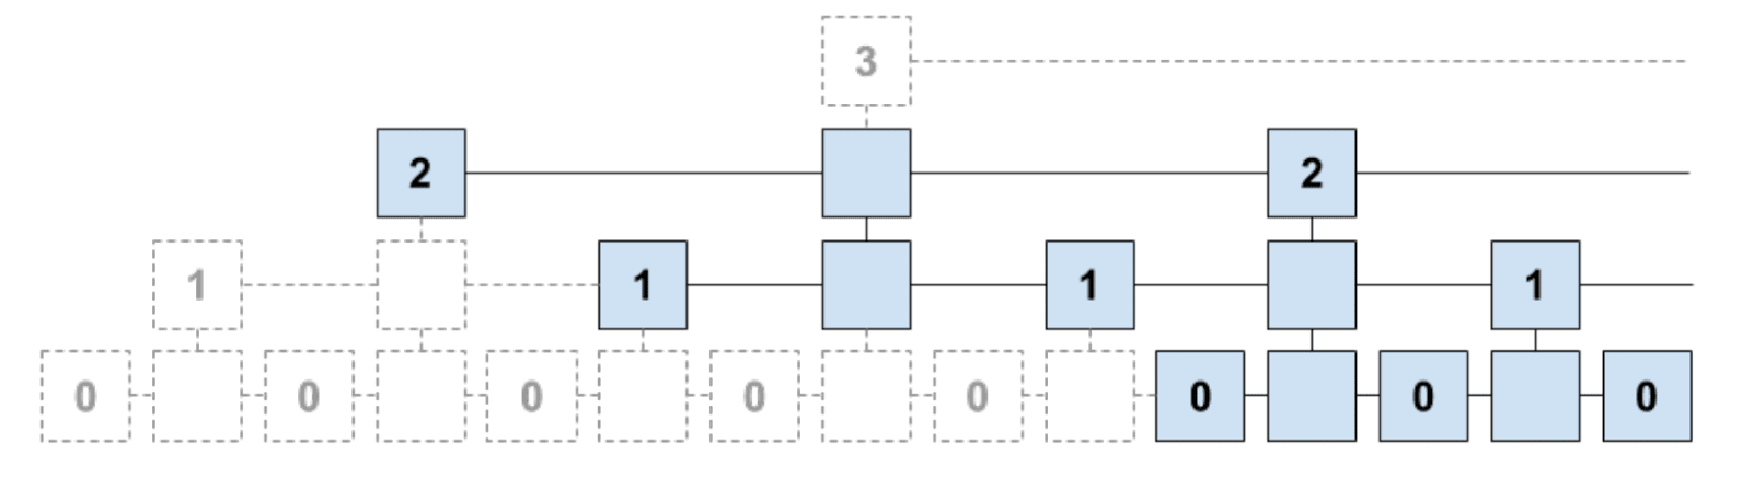
\includegraphics[width=0.8\columnwidth]{figures/suffix.pdf}
	\end{center}
	\caption{Superblock NIPoPoW proof prefix $\pi$ for $m = 3$~\cite{nipopows}.}
	\label{fig:suffix}
\end{figure}

\begin{algorithm}[h]
		\caption{\label{alg:suffix_prover_soft_fork}The Suffix Prover for the superblock NIPoPoW protocol~\cite{nipopows}}
		\begin{algorithmic}[1]
				\Function{\sf Prove$_{m,k}$}{$\chain$}
					\Let{B}{\chain[0]}
					\For{$\mu = \lvert \chain[-k].\textsf{interlink} \rvert$ down to $0$}
						\Let{\alpha}{\chain[{:}-k]\{B{:}\}\upchain^\mu}
						\Let{\pi}{\pi \cup \alpha}
						\Let{B}{\alpha[-m]}
					\EndFor
					\Let{\chi}{\chain[-k{:}]}
					\State\Return$\pi\chi$
				\EndFunction
		\end{algorithmic}
\end{algorithm}

\subsection{The Verifier}
The suffix verifier is given in Algorithm~\ref{alg:suffix_verifier_soft_fork} and consists of two functions and an operator definition. Function $\mathsf{Verify}$ forms a generic verifier for any protocol-specific proof comparison operator $\leq_m$. This proof comparison operator is specifically instantiated for the superblock suffix verifier and utilizes the supporting function $\mathsf{best\text{-}arg}$.

The verifier algorithm is parameterized by a chain predicate $\mathcal{Q}$ and the security parameters $k, m$. The verifier receives several proofs from different provers which are represented as a collection of proofs $\mathcal{P}$. We consider that at least one received is constructed by an honest prover. Iterating over $\mathcal{P}$ the verifier extracts the best one.

As already described, each proof is a  valid chain considering the interlink pointers. For an honest prover the proof contains a subset of blocks of the adopted chain. Proofs consist of two parts $\pi$ and $\chi$; $\pi$ is the proof prefix and $\chi$ the proof suffix. For honest provers, $\chi$ contains the last $k$ blocks of the adopted chain, while $\pi$ contains a subset of superblocks selected as explained in the prover algorithm.

For each proof the verifier first checks its validity by ensuring that $\lvert \chi \rvert = k$ and that $(\pi, \chi)$ is an anchored chain ($\mathsf{validChain(\cdot)}$). The best known prefix is initialized with the genesis block. At each loop iteration the verifier compares the next candidate proof prefix $\pi$ against the currently known best prefix $\tilde{\pi}$ and updates both $\tilde{\pi}, \tilde{\chi}$ if needed. 

The $\geq_m$ operator performs the comparison of two proofs. It takes proofs $\pi_\mathcal{A}, \pi_B$ and return true if the first one is winning and false otherwise. It first computes the LCA block $b$ between the two proofs. Since the proofs are valid chains, parties $\mathcal{A}, B$ have common underlying chain up to block $b$, so it suffices to compare the proofs for the diverging chains after $b$. The verifier selects as level of comparison of each proof the best possible argument by calling the $\mathsf{best\text{-}arg}$ function. In essence, the verifier selects the level containing the greatest amount of proof-of-work for each proof. This best argument selection by the verifier is called the \emph{principle of charity}. To find the best argument the verifier parses the proof one level at a time, weights the corresponding superblocks and selects the one resulting to the highest total PoW. The weighting of a $\mu-$superchain is performed by estimating the underlying number of blocks as $2^\mu \lvert \pi \upchain^\mu \{b:\} \rvert$. As discussed, the highest possible score across all levels is returned. Once the best argument of both proofs is known, they are directly compared and the winner returned. An advantage is given to first proof in case of a tie by using $\geq$ operator favoring $\mathcal{A}$. At the end of the loop the verifier will have determined the best proof $\tilde{\pi}, \tilde{\chi}$.

Note that $\chi$ might be needed for the final predicate evaluation but does not aprticipate in any comparison since it is of constant and equal size for any valid proof. We will prove that this proof will belong to an honest prover with high probability in the next section. 

\begin{algorithm}[h]
		\caption{\label{alg:suffix_verifier_soft_fork}The Suffix Verifier for the superblock NIPoPoW protocol~\cite{nipopows}}
		\begin{algorithmic}[1]
				\Function{\sf Verify$^{\mathcal{Q}}_{m,k}$}{$\mathcal{P}$}
					\Let{\tilde{\pi}}{(Gen)}
					\For{$(\pi, \chi) \in \mathcal{P}$}
						\If{$\text{validChain(\pi\chi)} \wedge \lvert \chi \rvert = k \wedge \pi \geq_m \tilde{\pi}$}
							\Let{\tilde{\pi}}{\pi}
							\Let{\tilde{\chi}}{\chi}
						\EndIf
					\EndFor
					\State\Return$\tilde{\mathcal{Q}}(\tilde{\chi})$
				\EndFunction
				\vspace{3mm}
				\Operator{$\pi_\mathcal{A} \geq_m \pi_b$}
					\Let{b}{(\pi_\mathcal{A} \cap \pi_B)[-1]}
					\State\Return$\mathsf{best\text{-}arg}_m(\pi_\mathcal{A}, b) \geq \mathsf{best\text{-}arg}_m(\pi_B, b)$
				\EndOperator
				\vspace{3mm}
				\Function{\sf best-arg$_m$}{$\pi, b$}
					\Let{M}{\{ \mu: \lvert \pi \upchain^\mu \{b:\} \rvert \geq m \} \cup \{0\}}
					\State\Return$\text{max}_{\mu \in M}\{2^\mu \cdot \lvert \pi \upchain^\mu \{b:\} \rvert \}$
				\EndFunction
		\end{algorithmic}
\end{algorithm}
 
\subimport{./}{security_proof_suffix.tex} 
 
\section{Infix Proofs}

\section{Succinctness}
 
